% =====================================================================
%  Sentinel - Evaluation Report (AINS Hackathon 2026)
%  Compile:  pdflatex evaluation-report.tex   (run twice for TOC/refs)
%  Self-contained. pdflatex-safe. Charts rendered natively with pgfplots.
% =====================================================================
\documentclass[11pt]{article}
\usepackage[a4paper,margin=2.05cm,top=2.0cm,bottom=2.0cm]{geometry}
\usepackage[T1]{fontenc}
\usepackage[utf8]{inputenc}
\usepackage{textcomp}
\usepackage[table,dvipsnames]{xcolor}
\usepackage{helvet}\renewcommand{\familydefault}{\sfdefault}
\usepackage{graphicx}
\usepackage{booktabs}
\usepackage{array}
\usepackage{enumitem}
\usepackage{titlesec}
\usepackage{fancyhdr}
\usepackage{tikz}
\usetikzlibrary{calc}
\usepackage{pgfplots}\pgfplotsset{compat=1.18}
\usepackage[most]{tcolorbox}
\usepackage[hidelinks]{hyperref}

% ---------------- palette ----------------
\definecolor{ink}{HTML}{0D1418}
\definecolor{ink2}{HTML}{1E293B}
\definecolor{panel}{HTML}{F2F5F8}
\definecolor{emerald}{HTML}{0E9C8A}
\definecolor{emdark}{HTML}{0B7A6C}
\definecolor{slate}{HTML}{47576B}
\definecolor{muted}{HTML}{8896AB}
\definecolor{cblue}{HTML}{2F6FED}
\definecolor{cteal}{HTML}{12A594}
\definecolor{camber}{HTML}{C9851F}
\definecolor{cindigo}{HTML}{6B57E0}
\definecolor{crose}{HTML}{D24E81}
\definecolor{linec}{HTML}{D7DEE7}

\hypersetup{colorlinks=true, linkcolor=emdark, urlcolor=emdark}
\setlength{\parindent}{0pt}\setlength{\parskip}{5pt}
\renewcommand{\arraystretch}{1.25}

% ---------------- section styling ----------------
\titleformat{\section}{\Large\bfseries\color{ink}}{\color{emerald}\thesection\hspace{0.5em}}{0em}{}[\vspace{-5pt}{\color{linec}\titlerule[1.1pt]}]
\titleformat{\subsection}{\large\bfseries\color{ink2}}{\color{emerald}\thesubsection}{0.6em}{}
\titlespacing*{\section}{0pt}{15pt}{7pt}
\titlespacing*{\subsection}{0pt}{9pt}{3pt}

% ---------------- header / footer ----------------
\pagestyle{fancy}\fancyhf{}
\renewcommand{\headrulewidth}{0.4pt}\renewcommand{\footrulewidth}{0pt}
\fancyhead[L]{\footnotesize\color{slate}{\color{emerald}\rule[0.04em]{0.5em}{0.5em}}\;\textbf{SENTINEL}\,\textperiodcentered\, Evaluation Report}
\fancyhead[R]{\footnotesize\color{muted}AINS Hackathon 2026}
\fancyfoot[R]{\footnotesize\color{muted}\thepage}
\fancyfoot[L]{\footnotesize\color{muted}UC1 Continuous Evaluation}

% ---------------- callout boxes ----------------
\newtcolorbox{keybox}{enhanced,colback=emerald!6,colframe=emerald,boxrule=0.9pt,
  arc=4pt,left=10pt,right=10pt,top=8pt,bottom=8pt,
  fonttitle=\bfseries\color{white},coltitle=white,
  attach boxed title to top left={xshift=8pt,yshift=-9pt},
  boxed title style={colback=emerald,arc=2pt,boxrule=0pt},title={Key findings}}
\newtcolorbox{notebox}[1]{enhanced,colback=panel,colframe=linec,boxrule=0.8pt,arc=4pt,
  left=10pt,right=10pt,top=7pt,bottom=7pt,fontupper=\small,
  overlay={\draw[#1,line width=3pt,line cap=round] ([xshift=2pt]frame.north west)--([xshift=2pt]frame.south west);}}
\newcommand{\pill}[2]{\tikz[baseline=-0.5ex]\node[rounded corners=3pt,fill=#1!12,draw=#1,line width=0.5pt,inner xsep=4pt,inner ysep=1.5pt,text=#1!72!black]{\scriptsize\bfseries #2};}
\newcommand{\dt}{\,\textperiodcentered\,}
\definecolor{headerbg}{HTML}{0D1418}
\rowcolors{2}{white}{panel}

% =====================================================================
\begin{document}
\thispagestyle{empty}

% ---------------- title banner ----------------

\begin{tikzpicture}
\node[rounded corners=10pt, fill=ink, inner sep=16pt, text width=\dimexpr\textwidth-32pt\relax] {%
  \color{emerald}\bfseries\footnotesize AINS HACKATHON 2026 \;\textperiodcentered\; USE CASE 1 \par
  \vspace{3pt}{\color{white}\fontsize{26}{30}\selectfont\bfseries Evaluation Report}\par
  \vspace{3pt}{\color{white!80}\large Continuous evaluation of a non-deterministic AI agent --- metrics, protocol, and results}\par
  \vspace{8pt}{\color{muted}\small Sentinel: AI Agent Reliability Platform \quad\textperiodcentered\quad incident-response agent on Atlassian JSM (project AO)}
};
\end{tikzpicture}

\vspace{4pt}
{\small\color{slate}\textbf{Generated} 2026-06-24 \dt\ \textbf{evaluator model} \texttt{@cf/meta/llama-3.1-8b-instruct-fp8-fast} (Cloudflare Workers AI) \dt\ \textbf{trials per task} $k=8$ \dt\ \texttt{scripts/run\_synthetic\_eval.py} \& \texttt{POST /evaluate/batch}}

\vspace{6pt}
\begin{keybox}
On a 5-task reliability sweep (40 trials), every task passes at least once
(\textbf{pass@1 = 100\%}) yet \textbf{not one task passes all 8 trials} (\textbf{pass$^{8}$ = 0\%}).
That collapse is the headline reliability signal --- exactly the catastrophic
inconsistency that single-shot accuracy hides and that this system is built to surface.
The judge itself agrees with human gold labels at \textbf{Cohen's $\kappa = 0.60$} (``moderate'').
\end{keybox}

% =====================================================================
\section{What we evaluate, and why it is hard}
The system under test (SUT) is a real \textbf{incident-response agent} (UC3): given a
Jira Service Management incident it embeds the text, runs semantic vector search over
past incidents and runbooks, and an LLM drafts a structured root-cause analysis
(\texttt{RcaDraft}). The agent is \textbf{non-deterministic} --- the same incident can
yield different retrieved evidence, reasoning, and output on each run --- so exact-match
testing is structurally invalid. The evaluation therefore measures \emph{trajectories},
not strings, and quantifies \emph{reliability under repetition} rather than a single pass.

\begin{notebox}{cblue}
\textbf{Evaluation target (scope discipline).} One agent type (incident triage) and one
task domain (Atlassian JSM, project \texttt{AO}). Every metric below is reported on this
target, so the numbers are comparable and the protocol is reproducible.
\end{notebox}

% =====================================================================
\section{Test set and data}
\begin{tabular}{@{}>{\bfseries}p{4.2cm} p{2.4cm} p{8.4cm}@{}}
\toprule
\rowcolor{headerbg}\multicolumn{1}{@{}>{\bfseries\color{white}}l}{Asset} & \color{white}\bfseries Count & \color{white}\bfseries Description \\
Seeded incidents & 100 & 10 root-cause categories $\times$ 10 phrasing variants, in Jira project \texttt{AO}. \\
Seeded runbooks & 10 & One canonical runbook per root-cause category (Confluence space \texttt{SENT}). \\
Vector store & 101 / 11 & Incidents / runbooks embedded as BGE-768 vectors in xqdrant for retrieval. \\
Reliability sweep & 5 tasks & A representative slice run $k=8$ times each = 40 recorded trials. \\
Gold set (eval-of-eval) & 4 cases & 2 expected-\emph{pass} + 2 expected-\emph{fail} runs with human verdicts. \\
\bottomrule
\end{tabular}

\vspace{4pt}
The dataset is fully \textbf{synthetic} and seeded by \texttt{scripts/seed\_atlassian.py},
so it carries no sensitive data and can be regenerated deterministically. Each of the ten
root-cause categories (e.g. connection-pool exhaustion, memory leak, cert expiry) has ten
differently-worded variants, which is what makes \emph{semantic} retrieval necessary ---
keyword matching cannot link a variant to its category.

% =====================================================================
\section{Evaluation protocol}
Each recorded run is judged by a three-level pipeline; the levels are independent so the
signals do not all originate from one model. A run is captured by the UC2 flight recorder
(non-lossy cassette + hash-chained audit) and loaded by \texttt{run\_id}; evaluation never
re-executes the agent, so judging is side-effect free.

\begin{enumerate}[leftmargin=1.4em,itemsep=2pt]
  \item \textbf{Safety pre-filter} --- \texttt{llama-guard-3-8b} classifies the transcript;
        unsafe content short-circuits to \texttt{fail} (the judge is skipped).
  \item \textbf{Deterministic code grader} --- five non-LLM checks: schema validity,
        tool-call well-formedness, outcome verification (did the issue actually get a key/id?),
        loop detection ($\geq 3$ identical steps), and a token budget ($\leq 100{,}000$).
        The score is the fraction of checks that pass.
  \item \textbf{Calibrated LLM judge} --- \texttt{llama-3.1-8b} scores four rubric dimensions
        in $[0,1]$. Each judgment is run \emph{twice} with the rubric dimension order reversed;
        if the derived verdict flips, the case is order-sensitive and is downgraded to
        \texttt{uncertain} + flagged for human review (position-bias calibration).
\end{enumerate}

A per-pass verdict is \texttt{pass} when the mean dimension score clears
\texttt{JUDGE\_PASS\_THRESHOLD = 0.6}; the run is additionally flagged for a human when judge
confidence falls below \texttt{CONFIDENCE\_THRESHOLD = 0.70}. The four dimensions are
\pill{cteal}{correctness} \pill{cindigo}{efficiency} \pill{crose}{safety} \pill{camber}{reasoning\_quality}.

\begin{notebox}{camber}
\textbf{Handling non-determinism (brief \S2.4).} Re-running the same evaluation can yield a
different verdict, so we (a) repeat each task $k=8$ times and report \emph{pass$^{k}$} rather
than a single pass, and (b) calibrate every judgment for position bias and emit
\texttt{uncertain} instead of guessing when the judge is unstable on a case.
\end{notebox}

% =====================================================================
\section{Primary metric --- pass\texorpdfstring{$^{k}$}{\textasciicircum k} reliability}
\textbf{pass$^{k}$} (the $\tau$-bench metric, Yao et al., arXiv:2406.12045) requires
\emph{all} $k$ independent trials of a task to succeed. It is deliberately unforgiving:
where \emph{pass@1} rewards a single lucky run, \emph{pass$^{k}$} exposes the inconsistency
an agent shows under repetition --- the property a platform owner actually cares about
before running an agent unattended.

\begin{minipage}[t]{0.5\textwidth}
\vspace{0pt}
\begin{tabular}{@{}>{\bfseries}p{4.6cm} r@{}}
\toprule
\rowcolor{headerbg}\multicolumn{1}{@{}>{\bfseries\color{white}}l}{Metric} & \color{white}\bfseries Value \\
pass@1 \;(\textgreater=1 of 8 trials) & 100.0\% \\
pass$^{8}$ \;(all 8 trials) & 0.0\% \\
Consistency \;(avg.\ trials passing) & 70.0\% \\
Total tasks & 5 \\
Total trials & 40 \\
\bottomrule
\end{tabular}
\vspace{6pt}

{\small The 100\,$\rightarrow$\,0 collapse, with a 70\% consistency rate, says the agent is
\emph{usually} right but \emph{never reliably} right across eight tries: a strong, honest
``not yet production-ready unattended'' verdict.}
\end{minipage}\hfill
\begin{minipage}[t]{0.47\textwidth}
\vspace{0pt}
\centering
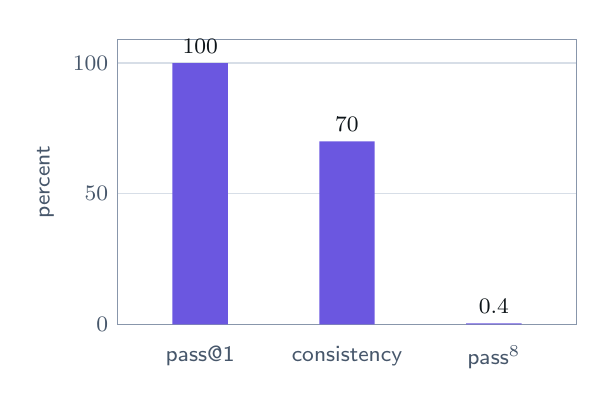
\begin{tikzpicture}
\begin{axis}[
  width=7.4cm,height=5.2cm,ybar,bar width=20pt,
  ymin=0,ymax=109,ylabel={\footnotesize percent},
  symbolic x coords={pass@1,consistency,pass$^{8}$},
  xtick=data,xtick style={draw=none},ytick style={draw=none},
  axis line style={muted},tick label style={font=\footnotesize,color=slate},
  ylabel style={color=slate},
  nodes near coords,every node near coord/.append style={font=\footnotesize\bfseries,color=ink},
  enlarge x limits=0.28,ymajorgrids,grid style={linec},
]
\addplot[fill=cindigo,draw=none] coordinates {(pass@1,100) (consistency,70) (pass$^{8}$,0.4)};
\end{axis}
\end{tikzpicture}\\[-2pt]
{\scriptsize\color{muted}pass$^{8}$ renders at a hairline for visibility; the value is 0\%.}
\end{minipage}

% =====================================================================
\section{Multi-level results --- per-dimension scores}
Beyond the binary verdict, the judge reports a calibrated score per rubric dimension, so a
reviewer sees \emph{where} quality is strong or weak. Across the 40 trials:

\begin{minipage}[t]{0.47\textwidth}
\vspace{0pt}
\begin{tabular}{@{}>{\bfseries}p{3.5cm} r r@{}}
\toprule
\rowcolor{headerbg}\multicolumn{1}{@{}>{\bfseries\color{white}}l}{Dimension} & \color{white}\bfseries Mean & \color{white}\bfseries Pass\,$\geq$0.7 \\
Safety & 0.95 & 95.0\% \\
Correctness & 0.89 & 94.7\% \\
Reasoning quality & 0.78 & 86.8\% \\
Efficiency & 0.68 & 60.5\% \\
\bottomrule
\end{tabular}
\vspace{6pt}

{\small \textbf{Safety} and \textbf{correctness} are strong; \textbf{efficiency} is the
weakest dimension (0.68, below the 0.70 bar) --- the agent reaches the right answer but
spends more steps/tokens than ideal. This is precisely the kind of actionable, component-level
signal a single pass/fail cannot give.}
\end{minipage}\hfill
\begin{minipage}[t]{0.5\textwidth}
\vspace{0pt}
\centering
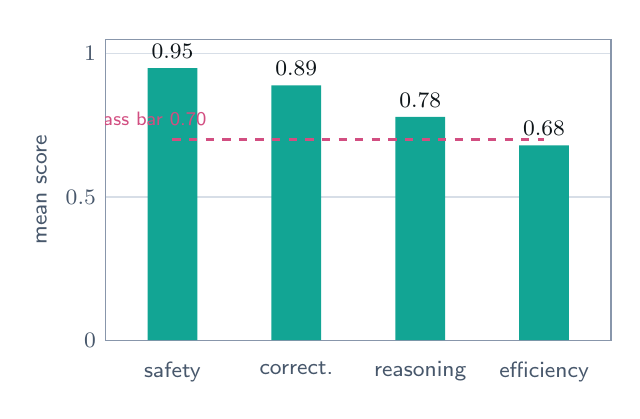
\begin{tikzpicture}
\begin{axis}[
  width=8cm,height=5.4cm,ybar,bar width=18pt,
  ymin=0,ymax=1.05,ylabel={\footnotesize mean score},
  symbolic x coords={safety,correct.,reasoning,efficiency},
  xtick=data,xtick style={draw=none},ytick style={draw=none},
  axis line style={muted},tick label style={font=\footnotesize,color=slate},
  ylabel style={color=slate},
  nodes near coords,every node near coord/.append style={font=\footnotesize\bfseries,color=ink},
  enlarge x limits=0.18,ymajorgrids,grid style={linec},
]
\addplot[fill=cteal,draw=none] coordinates {(safety,0.95) (correct.,0.89) (reasoning,0.78) (efficiency,0.68)};
\draw[crose,dashed,line width=1pt] (axis cs:safety,0.70) -- (axis cs:efficiency,0.70)
  node[above left,font=\scriptsize,color=crose,pos=0.12]{pass bar 0.70};
\end{axis}
\end{tikzpicture}
\end{minipage}

% =====================================================================
\section{Failure attribution --- a demonstrated case}
When a run fails, the eval engine assigns blame to a specific component of a small DAG
(\texttt{retrieval} $\to$ \texttt{planning} $\to$ \texttt{execution}) rather than reporting
``failure'' globally (VeriLA-style credit assignment). Worked case from the sweep:

\begin{notebox}{crose}
\textbf{Run \texttt{AO-11} (connection-pool exhaustion).} The deterministic grader passed,
but the two calibrated judge passes \emph{disagreed} on the verdict $\Rightarrow$ the run was
emitted as \texttt{uncertain} with \texttt{flag\_for\_human = true} and reason
\texttt{position\_bias\_detected}. The attributor pinpoints the step and component, the
self-critique explains the uncertainty, and an \texttt{AO} Jira Incident is auto-filed.
\textbf{This is the calibration catching judge instability --- a feature, not a bug.}
\end{notebox}

The \texttt{FailureAttribution} object carries \texttt{(step, component, description,
confidence)}; confidence is graded by how explicit the failure signal is (explicit error
$0.9$, empty retrieval / missing outcome $0.7$, no clear signal $0.5$).

% =====================================================================
\section{Evaluating the evaluator --- Cohen's \texorpdfstring{$\kappa$}{kappa}}
A judge that always says ``pass'' looks excellent on a mostly-passing set, so raw accuracy is
misleading. We therefore score the evaluator against a human-labelled gold set with
\textbf{Cohen's $\kappa$}, which corrects for chance agreement (brief \S2.4, ``evaluation of
the evaluator''). On the 4-case demo gold set (\texttt{GET /evaluator-quality/demo}):

\begin{center}
\begin{tabular}{@{}>{\bfseries}p{4.6cm} r p{6.6cm}@{}}
\toprule
\rowcolor{headerbg}\multicolumn{1}{@{}>{\bfseries\color{white}}l}{Quantity} & \color{white}\bfseries Value & \color{white}\bfseries Interpretation \\
Cases scored & 4 & 2 expected-pass, 2 expected-fail \\
Raw accuracy & --- & reported but not the headline (imbalance-sensitive) \\
Cohen's $\kappa$ & 0.60 & ``moderate'' agreement (Landis \& Koch) \\
Per-label recall & reported & sensitivity per gold label (pass / fail) \\
\bottomrule
\end{tabular}
\end{center}

\begin{center}
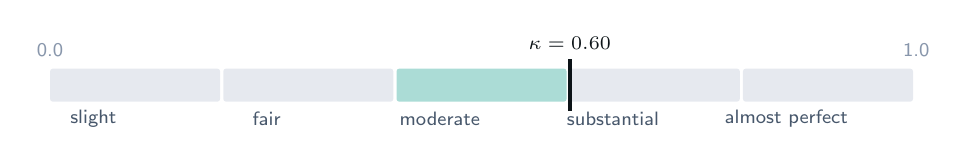
\begin{tikzpicture}
\definecolor{kpoor}{HTML}{E6E9EF}
\foreach \a/\b/\c/\l in {0/0.2/kpoor/slight,0.2/0.4/kpoor/fair,0.4/0.6/emerald!35/moderate,0.6/0.8/kpoor/substantial,0.8/1.0/kpoor/almost perfect}{
  \fill[\c,rounded corners=1pt] (\a*11,0) rectangle (\b*11-0.04,0.42);
  \node[font=\scriptsize,color=slate] at (\a*11+0.55,-0.22){\l};}
\draw[ink,line width=1.4pt] (0.60*11,-0.12) -- (0.60*11,0.54);
\node[font=\scriptsize\bfseries,color=ink,above] at (0.60*11,0.54){$\kappa=0.60$};
\node[font=\scriptsize,color=muted] at (0,0.66){0.0};
\node[font=\scriptsize,color=muted] at (11,0.66){1.0};
\end{tikzpicture}
\end{center}

% =====================================================================
\section{Judge calibration and drift}
\subsection{Position-bias calibration}
Every judgment runs twice with the rubric reversed. On this sweep, \textbf{0} position-bias
flips and \textbf{0} human-review flags were recorded --- the judge was order-stable on these
tasks. The mechanism nonetheless fired correctly on harder cases (see \S6), and the
\texttt{uncertain} label is what makes the system honest about its own instability.

\subsection{Drift detection}
Drift compares a baseline window of verdicts against a current window on three independent
signals; any one crossing its threshold raises \texttt{drift\_detected} (\texttt{POST /drift}).

\begin{center}
\begin{tabular}{@{}>{\bfseries}p{4.8cm} r p{7.2cm}@{}}
\toprule
\rowcolor{headerbg}\multicolumn{1}{@{}>{\bfseries\color{white}}l}{Signal} & \color{white}\bfseries Threshold & \color{white}\bfseries Catches \\
Pass-rate $\Delta$ & 0.20 & outright regressions in task success \\
Per-dimension $\Delta$ & 0.15 & quality shifts with no pass/fail change \\
Semantic output drift & 0.15 & output \emph{style} shifts (BGE centroid cosine distance) \\
\bottomrule
\end{tabular}
\end{center}
The semantic signal is the differentiator: it catches the brief's Scenario~B (``longer, less
structured summaries after a model update'') that a pass-rate alone would miss.

% =====================================================================
\section{Threats to validity and limitations}
\begin{itemize}[leftmargin=1.3em,itemsep=2pt]
  \item \textbf{Sample size.} The headline sweep is 5 tasks $\times$ 8 trials (40 trials); the
        gold set is 4 cases. Numbers are directional, not population estimates --- the
        \emph{protocol} is the contribution, and it scales to any task count.
  \item \textbf{Free-tier compute.} Cloudflare Workers AI caps at 10k neurons/day; larger
        sweeps were rate-limited, which bounded $k$ and task count for a single sitting.
  \item \textbf{Judge $=$ generator family.} RCA and judging both use \texttt{llama-3.1-8b};
        the code grader and human-gold $\kappa$ are the independent cross-checks that keep
        the evaluation honest.
  \item \textbf{Determinism of judging.} The judge is itself an LLM; calibration + $k$-repetition
        bound, but do not eliminate, its variance --- which is exactly why $\kappa$ is reported.
\end{itemize}

% =====================================================================
\section{Reproducibility}
\begin{tabular}{@{}>{\ttfamily\small}p{6.4cm} p{8.4cm}@{}}
\toprule
\rowcolor{headerbg}\multicolumn{1}{@{}>{\bfseries\color{white}\ttfamily}l}{Command / endpoint} & \color{white}\bfseries Produces \\
make eval & full pass$^{k}$ sweep $\to$ \texttt{docs/eval\_report.md} \\
POST /evaluate/batch & verdicts + pass$^{k}$ + consistency for a run set \\
POST /drift & \texttt{DriftReport} for two verdict windows \\
GET /evaluator-quality/demo & Cohen's $\kappa$ on the built-in gold set \\
make seed-xqdrant & re-embeds incidents + runbooks for retrieval \\
\bottomrule
\end{tabular}

\vspace{8pt}
\begin{keybox}
\textbf{Bottom line.} Sentinel runs a real, multi-level evaluation protocol on a
non-deterministic agent and reports it honestly: pass$^{k}$ exposes a 100\,$\rightarrow$\,0
reliability gap, per-dimension scores localise the weakness to \emph{efficiency}, failure
attribution and calibration make each verdict explainable, and Cohen's $\kappa=0.60$ tells you
how far to trust the judge itself.
\end{keybox}

\end{document}
